\section{Simulation (z.B. Molekülsimulation (molecular dynamic) für die Pharma Industrie) mittels eines Quantencomputer}

\begin{enumerate}
    \item die Quantenwelle $\psi$ 'bewegt' sich (wir wissen nicht, wo $\psi$ liegt) im Raum (Abb. \ref{bloch}) und hat den Zustand $\ket{\psi}$
        (als Vektor/Pfeil dargestellt)
    \begin{SCfigure}[][h!]
        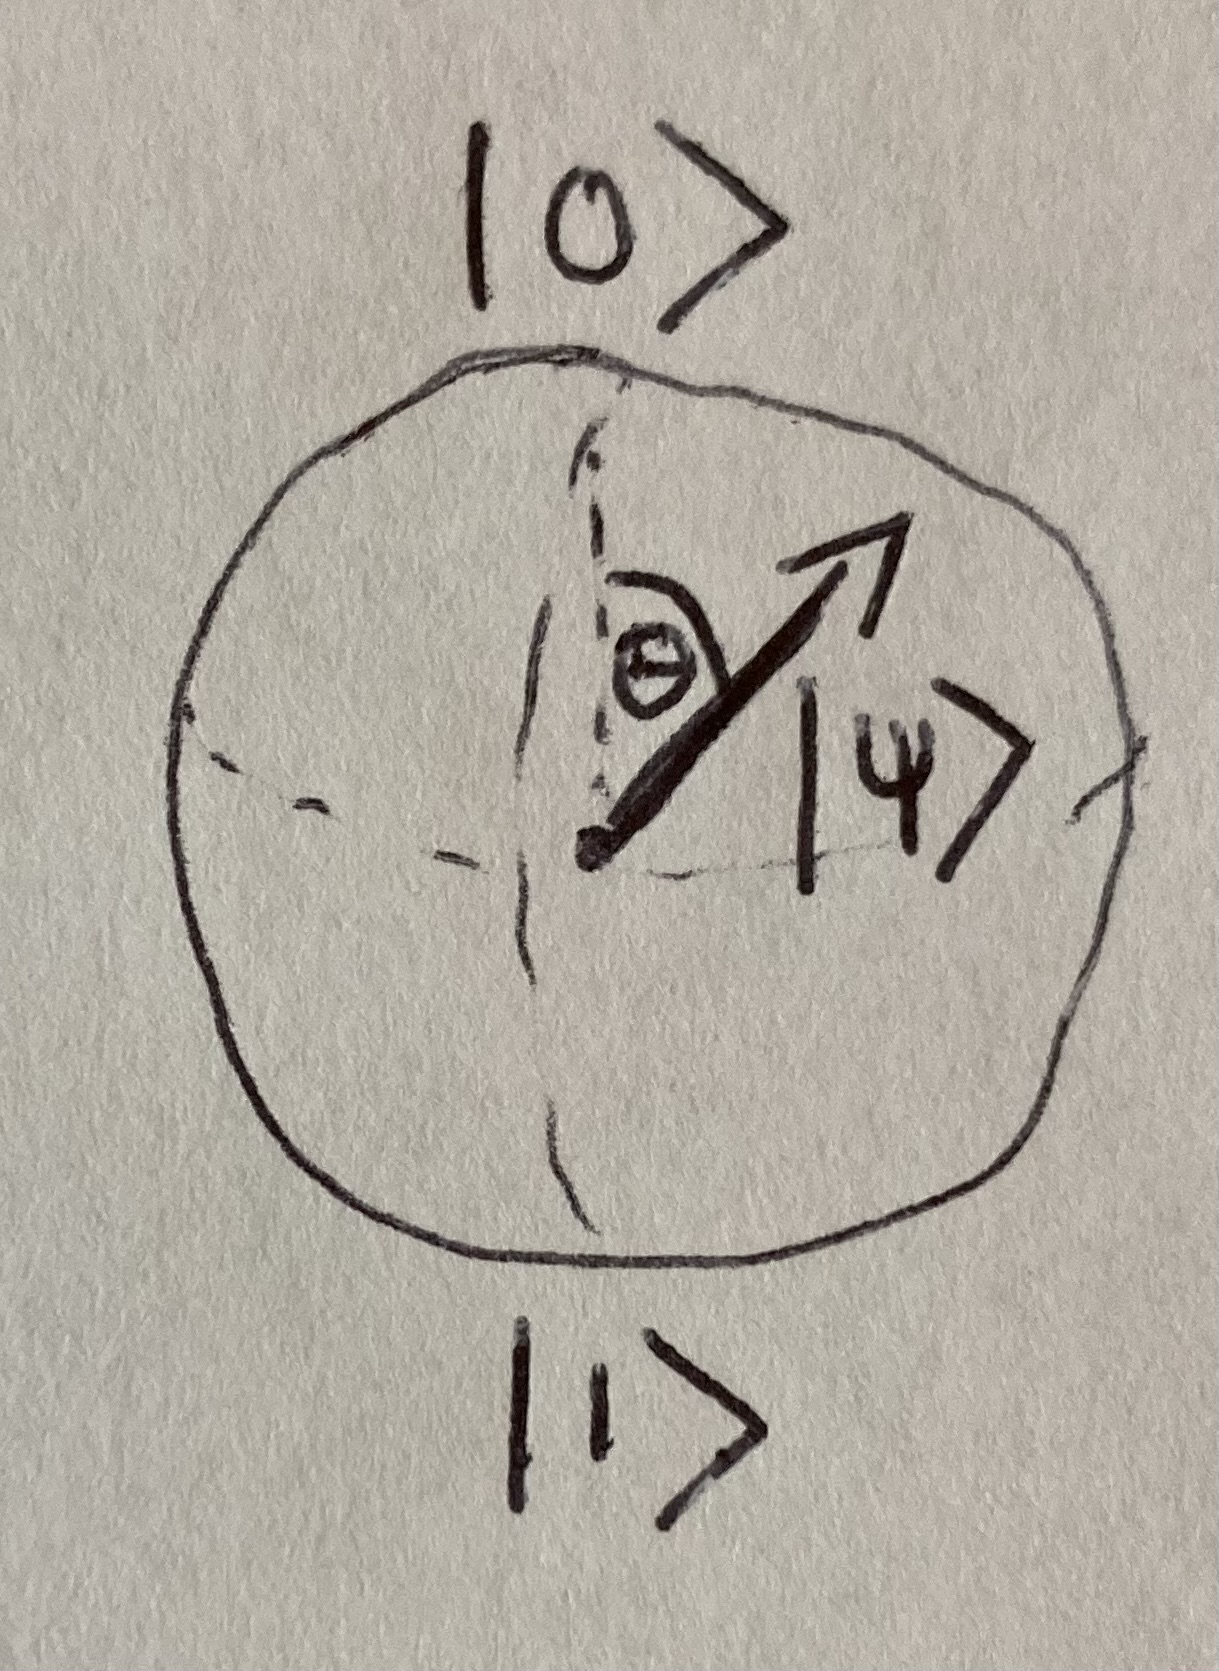
\includegraphics[width=0.35\textwidth]{bloch_kugel.png}
        \caption{Bloch-Kugel (zur Visualisierung eines 2 Zustände ($\ket{0}$ oder $\ket{1}$) Qubit), auf der
                    alle Zustände von $\ket{\psi}$ durch Punkte auf der Kugel Oberfläche beschrieben werden} 
        \label{bloch} 
    \end{SCfigure}
    \item Wir versuchen mathematisch eine Aussage zu machen, wie wahrscheinlich (Wahrscheinlichkeitsverteilung P(x) (Statistik)) es ist, dass $\ket{0}$
        oder $\ket{1}$ eintritt (z.B. P($\ket{0})$=0.7)):
        \begin{equation*}
            \psi(\vec{x})=\braket{\vec{x}|\psi}
        \end{equation*}
        mit $\ket{\vec{x}}=\ket{0}$ oder $\ket{1}$ (siehe Bloch-Kugel)
    \item Da sich die Quantenwelle 'bewegt', liegen die Zustände $\ket{0}$ und $\ket{1}$ $\underline{vor}$ der Messung
        in Superposition vor (\textbf{Gedankenexperiment}: Schrödinger Katze). Diese Superposition ist eine Teil der Kohärenzeigenschaft, worunter 
        die Überlagerung von Wellen und Teilchen Eigenschaft, sowie die Verschränkung auch fällt. Kohärenz und die damit 
        verbundene Zeitdauer (=Kohärenzzeit) erlaubt das Auftreten von quantenmechanischen Effekten und damit auch 
        die quantenmechanischen Berechnungen.
        \begin{equation*}
            \ket{\psi}=a\ket{0}+b\ket{1} 
        \end{equation*}
        (mit $\vert a\vert^2+\vert b\vert^2=1$)\\
        \underline{hier}:
        \begin{equation*}
            \ket{\psi}=\cos(0.5\theta)\ket{0}+e^{i\psi}\sin(0.5\theta)\ket{1}
        \end{equation*}
    \item Sobald wir messen, kollabiert $\psi$ auf einen messbaren Zustand ($\ket{0}$ oder $\ket{1}$) (seinen 'Eigenwert' $\lambda$). Die Superposition
        wird dabei zerstört, was eine Aufhebung der Köhrenz und damit verbundenes Ende der Quanteneffekte darstellt. Zusätzlich 
        kann die Superposition auch durch Wechselwirkung mit der Umgebung ungewollt zerstört werden.
    \item Beim Quantencomputer kann man $\underline{vor}$ der Messung (welche durch einen hermitischen Operator $\hat{A}, \hat{H}$ etc. erfolgt)
        den Zustand $\ket{\psi}$ durch Einsatz von Quantengatter noch ändern. Dies passiert durch Pulse von Mikrowellen auf den Qubit. 
        Quantengatter sind z.B.:
        \begin{enumerate}
            \item NOT Gatter
            \item Haddamard Gatter 
            \item Phasen Gatter
        \end{enumerate}
        Schaltet man mehrere Quantengatter hintereinander, bildet das den Quantenalgorithms, welcher oft auch quantum circuit
        bezeichnet wird. Dies ist momentan wie eine 'black box'. Die Algorithmen werden nach einen Trial and Error Prinzip entworfen,
        da man ja vorher nicht weiß, welche Lösung für das gestellte Problem die Richtige ist. Dies ist wie bei den Formeln der Quantenmechanik, 
        welche häufig auch nur erraten sind. Die Grundlage der Wirklichkeit ist nicht bekannt. Vlt. werden deshalb auch die Entwicklung von
        Quantenalgorithmen immer eine 'black box' bleiben. 
\end{enumerate}
Abschließend möchte ich noch sagen, dass beim Doppelspalt-Versuch wir auch die Atome/Moleküle nur mit ihren jeweiligen 
kohärenten Zustand $\ket{\psi}$ auf den Bildschirmdetektor schießen.\\
Die Kohärenzzeit muss erhöht werden, damit das Quantenverhalten nicht so schnell verloren geht.


